\documentclass[a4paper]{article}

%% Language and font encodings
\usepackage[english]{babel}
\usepackage[utf8x]{inputenc}
\usepackage[T1]{fontenc}
\usepackage{cite}

\usepackage{graphicx}
\usepackage{subcaption}
\usepackage{tikz}
\usepackage{pgfplots}
\usepackage{wrapfig}
\usepackage{cutwin}
\graphicspath{ {images/} }
\usetikzlibrary{intersections,decorations.pathreplacing,decorations.markings,calc}

%% Sets page size and margins
\usepackage[a4paper,top=3cm,bottom=2cm,left=2.5cm,right=2.5cm,marginparwidth=1.75cm]{geometry}

%% Useful packages
\usepackage{amsmath}
\usepackage{amsthm}
\usepackage{amssymb}
\newtheorem{prop}{Propostition}
\usepackage{tikz}
\usepackage{graphicx}
\usepackage{hyperref}
\usepackage{caption}
%\usepackage{subcaption}
\usepackage{float}
\captionsetup{font={small,it}}
\theoremstyle{definition}
\newcommand{\D}{\mathcal{D}}
\newcommand{\Z}{\mathbb{Z}}
\newcommand{\R}{\mathbb{R}}
\newcommand{\C}{\mathcal{C}}
\newcommand{\A}{\mathcal{A}}
\newcommand{\B}{\mathcal{B}}
\renewcommand{\L}{\mathcal{L}}
\renewcommand{\S}{\mathcal{S}}
\newcommand{\K}{\mathcal{K}}
\renewcommand{\O}{\mathcal{O}}
\renewcommand{\epsilon}{\varepsilon}
\newcommand{\dx}{\: \mathrm{d}}
\newcommand{\Scrystal}{\mathcal{S}_D^\#}
\newcommand{\KstarC}{(\mathcal{K}_D^{\#})^*}
\newcommand{\expl}[1]{\left[\text{\footnotesize \emph{#1}} \right]}
\newcommand{\ds}{\displaystyle}
\newcommand{\eqnref}[1]{(\ref {#1})}
\def\nm{\noalign{\medskip}}



\author{Erik Orvehed Hiltunen}

\begin{document}
\section{Introduction}
We consider acoustic wave propagation in a crystal with bubbles repeated in a periodic square lattice. It has previously been shown that such crystal exhibits a frequency bandgap, so waves with frequencies inside this bandgap will decay exponentially. By perturbing one bubble to a smaller radius, the resonance frequency of this bubble increases and will lie inside the bandgap. We therefore expect an exponentially localized mode in this defect.


\section{Problem statement}
Assume that a single bubble occupies $D$, which is a circle of radius $R_b$ and center at the origin. Let $\C = \cup_{n\in\Z^2}(D+n)$ be the periodic bubble crystal. Consider now a perturbed crystal, where $D$ is replaced by a defect circle $D_d$ of radius $R_d < R_b$. Let $\C_d = D_d \cup \left( \cup_{n\in\Z^2\setminus\{0,0\}} D+n \right)$ be the perturbed crystal and let $\epsilon = R_b-R_d$ be the perturbation of the radius. We consider the following problem:
\begin{equation} \label{eq:scattering}
\left\{
\begin{array} {ll}
	&\ds \nabla \cdot \frac{1}{\rho} \nabla  u+ \frac{\omega^2}{\kappa} u  = 0 \quad \text{in} \quad \R^2 \backslash \C_d, \\
	\nm
	&\ds \nabla \cdot \frac{1}{\rho_b} \nabla  u+ \frac{\omega^2}{\kappa_b} u  = 0 \quad \text{in} \quad \C_d, \\
	\nm
	&\ds  u_{+} -u_{-}  =0   \quad \text{on} \quad \partial \C_d, \\
	\nm
	& \ds  \frac{1}{\rho} \frac{\partial u}{\partial \nu} \bigg|_{+} - \frac{1}{\rho_b} \frac{\partial u}{\partial \nu} \bigg|_{-} =0 \quad \text{on} \quad \partial \C_d
\end{array}
\right.
\end{equation}
Here, $\partial/\partial \nu$ denotes the outward normal derivative and $|_\pm$ denote the limits from outside and inside $D$.  

Let
\begin{equation*} % \label{data1}
v = \sqrt{\frac{\kappa}{\rho}}, \quad v_b = \sqrt{\frac{\kappa_b}{\rho_b}}, \quad k= \frac{\omega}{v} \quad \text{and} \quad k_b= \frac{\omega}{v_b}
\end{equation*}
be respectively the speed of sound outside and inside the bubbles, and the wavenumber outside and inside the bubbles. We also introduce two dimensionless contrast parameters
\begin{equation*} % \label{data2}
\delta = \frac{\rho_b}{\rho} \quad \text{and} \quad \tau= \frac{k_b}{k}= \frac{v}{v_b} =\sqrt{\frac{\rho_b \kappa}{\rho \kappa_b}}. 
\end{equation*}

Let $\Gamma^k$ be the fundamental solution to the Helmholtz equation with wavenumber $k$, given by
\begin{equation*}
\Gamma^k(|x-y|) = -\frac{i}{4}H_0^{(1)}(k|x-y|).
\end{equation*}
Here $H_0^{(1)}$ is the Hankel function of the first kind. We will omit the superscript and simply write $H_0$ for this function. Let $\S_{D}^k$ be the single layer potential accociated to the free-space Green's function $\Gamma^k$, defined by
\begin{equation*}
\S_D^k[\phi](x) = \int_{\partial D} \Gamma^k(x,y)\phi(y) \dx \sigma(y), \quad x \in \R^2.
\end{equation*}
Let $G(x,y)$ be the Green's function corresponding to the periodic crystal $\C$, i.e. $G$ satisfies
\begin{equation*} \label{eq:G}
\Delta G + (k^2+(k_b^2-k^2)\chi(\C))G = \delta(x-y).
\end{equation*}
Let $\Scrystal$ be the single layer potential associated to $G$, i.e.
\begin{equation*}
\Scrystal[\phi](x) = \int_{\partial D} G(x,y)\phi(y) \dx \sigma(y) , \quad x \in \R^2.
\end{equation*}

We seek a solution $u(x)$ of the form
\begin{equation} \label{eq:sol}
u(x) = \begin{cases}
\S_{D_d}^{k_b}[\phi_1](x) \quad &x\in D_d, \\
\S_{D_d}^{k}[\phi_2](x) + S_D^k[\phi_3](x) & x\in D\setminus \bar{D}_d, \\
\Scrystal[\phi_4](x) & x \in \R^2\setminus \bar{D}.
\end{cases}
\end{equation}
A solution of this form satisfies the differential equation in \eqnref{eq:scattering}. To write the boundary conditions in equation \eqnref{eq:scattering} in terms of the boundary integral operators, we need the jump relations for the single layer potentials. For $S_D^k$, these are well known, but for $S_D^\#$ these must be computed.

\subsection{Jump relations for $\S_D^\#$}
The goal of this section is to derive the jump relations for the operator $\S_D^\#$ as $x$ tends to the boundary $\partial D$. Define the two operators 
\[(\K_D^{\#,\pm})^*[\phi](x) = \int_{\partial D}\frac{\partial G(x,y)}{\partial \nu(x)}\bigg|_{\pm} \phi(y)\dx \sigma(y),\]
where $\frac{\partial G(x,y)}{\partial \nu(x)}\big|_{\pm}$ are the values of $\frac{\partial G(x,y)}{\partial \nu(x)}$ as $x\rightarrow \partial D \pm$. Observe that the normal derivative of $G$ has a jump, so these values do not coincide. We have the following
\begin{prop} \label{prop:jump}
	The following jump relations hold for the single layer potential and its normal derivative:
\[\S_D^\#[\phi]\big|_+ = \S_D^\#[\phi]\big|_-\]
and
\[\frac{\partial \S_D^\#[\phi]}{\partial \nu} \bigg|_{\pm} = \pm \frac{c\phi}{2} + (\K_D^{\#,\pm})^* [\phi],\]
where $c$ is a material parameter given by
\[c = \frac{2}{\delta+1}.\]
\end{prop}
\begin{proof}
For $x$ close to $y$ on the boundary of a bubble, $|x-y|$ is small compared to the wavelength so we are in the quasi-static regime. We therefore expect the singularity of $G$ to be the same as the singularity of the Laplace Green's function $G_0(x,y)$, which is the solution to 
\begin{equation*}
\left\{
\begin{array}{ll}
	&\ds \Delta G_0 = \delta(x-y) \quad \text{in}\quad \R^2, \\
	&\ds \frac{1}{\rho}\frac{\partial G_0}{\partial \nu}\bigg|_+ - \frac{1}{\rho_b}\frac{\partial G_0}{\partial \nu}\bigg|_- = 0 \quad \text{in} \quad \partial D, \\
	&\ds G_0 \text{ satisfies Sommerfeld radiation condition.} 
\end{array}
\right.	
\end{equation*}
Set \begin{equation}\label{eq:gtilde}
\tilde{G}_0 = G_0-\Gamma^0,
\end{equation}
where $\Gamma^0(x,y)= \frac{-1}{2\pi}\ln(|x-y|)$ is the fundamental solution for the Laplace equation in $\R^2$. Then $\tilde{G}_0$ is the solution to the following problem
\begin{equation*}
\left\{
\begin{array}{ll}
&\ds \Delta \tilde{G}_0 = 0 \quad \text{in}\quad \R^2, \\
&\ds G_0\big|_+-G_0\big|_- = 0, \\
&\ds \frac{1}{\rho}\frac{\partial \tilde{G}_0}{\partial \nu}\bigg|_+ - \frac{1}{\rho}\frac{\partial \tilde{G}_0}{\partial \nu}\bigg|_- = (1-\delta)\frac{\partial \Gamma^0}{\partial \nu} \quad \text{in} \quad \partial D, \\
&\ds \tilde{G}_0 \text{ satisfies Sommerfeld radiation condition.} 
\end{array}
\right.	
\end{equation*}
It is well known that the solution to this problem is given by
\begin{equation*}
\tilde{G_0}(x,y) = \S_D^0 \left[\psi\right](x),
\end{equation*}
where
\begin{equation*}
\psi(z) = \left(\lambda I - \left( \K_D^0 \right)^*\right)^{-1} \left[ \frac{\partial\Gamma^0(z,y)}{\partial \nu(z)} \right] 
\end{equation*}
For a disk $D$, the operator $\left(\K_D^0\right)^*$ has an explicit expression
\begin{equation*}
\left(\K_D^0\right)^*[\phi](x) = \frac{1}{4\pi R_b}\int_{\partial D} \phi(y)\dx \sigma \quad \text{for all } x\in \partial D.
\end{equation*}
Furthermore, $\K_D^0$ is self-adjoint in this case. For $y$ outside $D$, the function $\Gamma^0(x,y)$ is harmonic as a function of $x\in D$. Therefore 
\begin{equation*}
\int_{\partial D} \frac{\partial \Gamma^0(x,y)}{\partial \nu(x)}\dx \sigma(x) = 0,
\end{equation*}
so it can easily be shown that 
\begin{equation*}
\int_{\partial D} \psi(x)\dx \sigma = 0,
\end{equation*}
and hence 
\begin{equation*}
\psi = \frac{1}{\lambda}\frac{\partial \Gamma^0}{\partial \nu}.
\end{equation*}
It follows that 
\begin{align*}
\tilde{G_0}(x,y) &= \frac{1}{\lambda}\S_D^0 \left[\frac{\partial \Gamma^0(z,y)}{\partial \nu(z)} \right](x) \\
&= \frac{1}{\lambda} \int_{\partial D} \Gamma^0(x,z) \frac{\partial \Gamma^0(z,y)}{\partial \nu(z)} \dx \sigma(z) \\
&=\frac{1}{\lambda}\mathcal{D}_D^0 \left[\Gamma^0(z,x)\right](y).
\end{align*}
Taking the limit $y\rightarrow \partial D+$ and using the jump relation for the double layer potential $\mathcal{D}_D^0$, we find
\begin{equation} \label{eq:gtildecomputated}
\tilde{G}_0(x,y) = -\frac{\Gamma^0(x,y)}{2\lambda} + \frac{1}{\lambda}\K_D^0\left[\Gamma^0(x,z)\right](y).
\end{equation}
Here, $\K_D^0\left[\Gamma^0(x,z)\right](y)$ is a bounded constant $C(x)$ with respect to $y$ (and actually equals $\frac{1}{2}\Gamma^0(x,0)$). Using equations \eqnref{eq:gtilde} and \eqnref{eq:gtildecomputed}, we find
\begin{equation*}
G_0(x,y) = c\Gamma^0(x,y) + C(x),
\end{equation*}
where 
\begin{equation*}
c = \frac{2}{\delta+1}.
\end{equation*}
Consequently, $G_0(x,y)-c\Gamma(x,y)$ is smooth, so also for the crystal Green's function $G(x,y)-c\Gamma(x,y)$ is smooth. 

The jump relations now follow by splitting the integral in $\S_D^\#$ to two integrals, with kernels $G(x,y)-c\Gamma^0(x,y)$ and $c\Gamma^0(x,y)$ respectively, and using the standard jump relations for $\S_D^0$. Explicitly, we have
\begin{align*}
\lim_{x\rightarrow \partial D \pm} \S_D^\#[\phi](x) &= \lim_{x\rightarrow \partial D \pm} \int_{\partial D} G(x,y) \phi(y)\dx \sigma(y) \\ 
&= \lim_{x\rightarrow \partial D \pm} \int_{\partial D} \left(G(x,y)-c\Gamma^0(x,y)\right) \phi(y)\dx \sigma(y) +  \lim_{x\rightarrow \partial D \pm} \int_{\partial D} c\Gamma^0(x,y) \phi(y)\dx \sigma(y)\\ 
&= \int_{\partial D}\left(G(x_0,y)-c\Gamma^0(x_0,y)\right) \phi(y)\dx \sigma(y) +   \int_{\partial D} c\Gamma^0(x_0,y) \phi(y)\dx \sigma(y)\\ 
&= \S_D^\#[\phi](x_0), \quad x_0 \in \partial D
\end{align*} 
and \marginpar{\footnotesize Really simple computations but nasty formulas, do we need this?}
\begin{align*}
\lim_{x\rightarrow \partial D \pm} \frac{\partial \S_D^\#[\phi](x)}{\partial \nu} &= \lim_{x\rightarrow \partial D \pm} \frac{\partial}{\partial \nu}\int_{\partial D} G(x,y) \phi(y)\dx \sigma(y) \\ 
&= \lim_{x\rightarrow \partial D \pm} \frac{\partial}{\partial \nu}\int_{\partial D} \left(G(x,y)-c\Gamma^0(x,y)\right) \phi(y)\dx \sigma(y) +  \lim_{x\rightarrow \partial D \pm} \frac{\partial}{\partial \nu}\int_{\partial D} c\Gamma^0(x,y) \phi(y)\dx \sigma(y)\\ 
&= \int_{\partial D}\frac{\partial}{\partial \nu(x_0)}\left(G(x_0,y)-c\Gamma^0(x_0,y)\right)\bigg|_{\pm} \phi(y)\dx \sigma(y) \pm \frac{c\phi(x_0)}{2} + \int_{\partial D} \frac{\partial}{\partial \nu(x_0)}c\Gamma^0(x_0,y) \phi(y)\dx \sigma(y)\\ 
&= \pm \frac{c\phi(x_0)}{2} + \K_D^{\#,\pm} [\phi](x_0), \quad x_0 \in \partial D.
\end{align*} 
\end{proof}

\subsection{Boundary integral formulation}
Using Proposition \ref{prop:jump} and the standard jump conditions for $\S_D^0$, the boundary conditions in \eqnref{eq:scattering} implies that the layer densities $\phi_i,\ i=1,2,3,4$ in \eqnref{eq:sol} satisfy the system of boundary integral equations
\[\A(\omega, \delta)\Phi = 0,\] where
\begin{equation} \label{eq:A}
\A(\omega, \delta) = 
\begin{pmatrix}
\S_{D_d}^{k_b} &  -\S_{D_d}^{k} & -\S_{D_d,D}^{k} & 0 \\
0 & \S_{D,D_d}^k & \S_{D}^k & -\Scrystal \\
-\frac{1}{2}I+ (\K_{D_d}^{k_b})^*& -\delta\left( \frac{1}{2}I+ (\K_{D_d}^{k})^*\right) & -\delta \frac{\partial \S_{D_d,D}^{k}}{\partial \nu} & 0 \\
0 & \frac{\partial \S_{D,D_d}^{k}}{\partial \nu} & -\frac{1}{2}I+ (\K_D^{k})^* & -\left( \frac{c}{2}I+ \left(\K_D^{\#,+}\right)^*\right)
\end{pmatrix}, 
\ \text{and}  \ \Phi= 
\begin{pmatrix}
\phi_1\\
\phi_2 \\
\phi_3 \\
\phi_4
\end{pmatrix}.
\end{equation}
Here the operator $\S_{D_d,D}^{k} = \S_{D}^{k}|_{x\in \partial D_d}$ is the restriction of $\S_{D}^{k}$ onto $\partial D_d$ and similarly for $\S_{D,D_d}^{k}$.

\section{Dilute regime}
ilute regime, i.e. the case when the bubble radius $R_b$ is small. In this case the effective medium theory for bubbly fluids applies. \cite{effectivemedium}

\section{Simplified problem}
By slightly shrinking the size of one bubble, we expect one localized mode, which quickly decays away from the perturbed bubble. The exponential decay means that the solution $u(x)$ is close to zero for $x$ away from the defect bubble. In this simplified problem, we assume that $u(x)=0$ for $|x|=R_b$, i.e. for $x$ on the large bubble $D$, and only consider the problem inside $D$. If this problem has a resonant mode, we expect the original problem to have a resonant mode corresponding to the defect bubble. We therefore consider the Dirichlet problem
\begin{equation} \label{eq:simple}
\left\{
\begin{array} {ll}
&\ds \nabla \cdot \frac{1}{\rho} \nabla  u+ \frac{\omega^2}{\kappa} u  = 0 \quad \text{in} \quad D \backslash D_d, \\
\nm
&\ds \nabla \cdot \frac{1}{\rho_b} \nabla  u+ \frac{\omega^2}{\kappa_b} u  = 0 \quad \text{in} \quad D_d, \\
\nm
&\ds  u_{+} -u_{-}  =0   \quad \text{on} \quad \partial D_d, \\
\nm
& \ds  \frac{1}{\rho} \frac{\partial u}{\partial \nu} \bigg|_{+} - \frac{1}{\rho_b} \frac{\partial u}{\partial \nu} \bigg|_{-} =0 \quad \text{on} \quad \partial D_d \\
&\ds u_- = 0 \quad \text{on} \quad \partial D.
\end{array}
\right .
\end{equation}
We seek the resonance frequencies, i.e. the frequencies $\omega$ such that equation \eqnref{eq:simple} has a non-trivial solution. This problem is solved numerically using two different methods. Similarly to equation \eqnref{eq:sol}, we seek a solution of the form 
\begin{equation} \label{eq:simplesol}
u(x) = \begin{cases}
\S_{D_d}^{k_b}[\phi_1](x) \quad &x\in D_d \\
\S_{D_d}^{k}[\phi_2](x) + S_D^k[\phi_3](x) & x\in D\setminus D_d,
\end{cases}
\end{equation}
satisfying $\tilde{\A}(\omega, \delta)\Phi = 0$, where
\begin{equation} \label{eq:simpleA}
\tilde{\A}(\omega, \delta) = 
\begin{pmatrix}
\S_{D_d}^{k_b} &  -\S_{D_d}^{k} & -\S_{D_d,D}^{k} \\
0 & \S_{D,D_d}^k & \S_{D}^k \\
-\frac{1}{2}I+ (\K_{D_d}^{k_b})^*& -\delta\left( \frac{1}{2}I+ \left(\K_{D_d}^{k}\right)^*\right) & -\delta \frac{\partial \S_{D_d,D}^{k}}{\partial \nu}
\end{pmatrix}, 
\ \text{and}  \ \Phi= 
\begin{pmatrix}
\phi_1\\
\phi_2 \\
\phi_3
\end{pmatrix}.
\end{equation}
The integral operators in $\tilde{\mathcal{A}}$ are discretized using Nyström's method and the smallest resonance frequency is computed using Muller's method. \cite{first}

To verify the solution, the problem is also solved using multipole expansions. Because the problem is a radially symmetric Helmholtz problem, the solution $u(x)$ can be written
\begin{equation*}
u(x) = \begin{cases}
\sum_{n=-\infty}^\infty a_n J_n(k_br)e^{in\theta} \quad &\text{if } r<R_d \\
\sum_{n=-\infty}^\infty \left(b_n J_n(kr) + c_n H_n(kr)\right) e^{in\theta}  &\text{if } r>R_d.
\end{cases}
\end{equation*}
Using the boundary conditions, we find that for every $n\in \Z$,
\begin{equation*} 
\begin{pmatrix}
J_n(k_bR_d) &  -J_n(kR_d) & -H_nkR_d) \\
k_bJ_n'(k_bR_d) & -\delta kJ_n'(kR_d) & -\delta k H'_n(kR_d)\\
0 & J_n(kR_b) & H_n(kR_b)
\end{pmatrix}
\begin{pmatrix}
a_n \\ b_n \\ c_n
\end{pmatrix} = 0.
\end{equation*}
We therefore seek the $\omega$ such that for some $n$, this system is not invertible. It is intuitively clear that the first resonant frequency will contain a factor with $n=0$, because the first resonance will have the least amount of oscillations. Thus, the lowest resonant frequency corresponds to the matrix
\begin{equation*} 
\begin{pmatrix}
J_0(k_bR_d) &  -J_0(kR_d) & -H_0(kR_d) \\
k_bJ_0'(k_bR_d) & -\delta kJ_0'(kR_d) & -\delta k H'_0(kR_d)\\
0 & J_0(kR_b) & H_0(kR_b)
\end{pmatrix}
\end{equation*}
being singular. This frequency is computed using Muller's method.
\begin{figure}[H]
	\centering
	\begin{minipage}[t]{0.45\linewidth}
	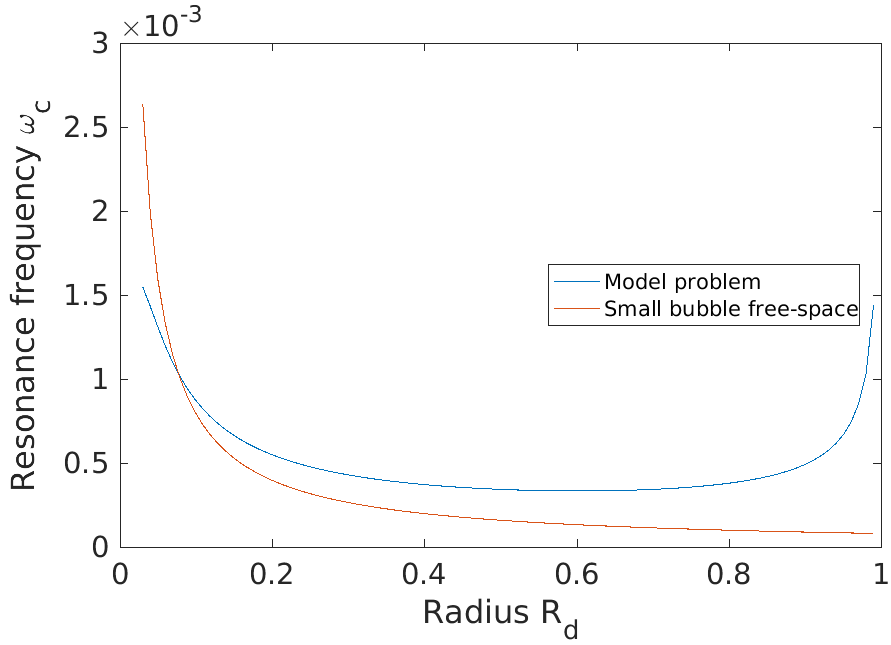
\includegraphics[scale=0.5]{../Model_problem/simpleSol.png}
	\caption{Resonance frequency for different defect radius $R_d$.}
	\label{fig:simpleSol}
	\end{minipage}
	\hspace{10pt}
	\begin{minipage}[t]{0.45\linewidth}
	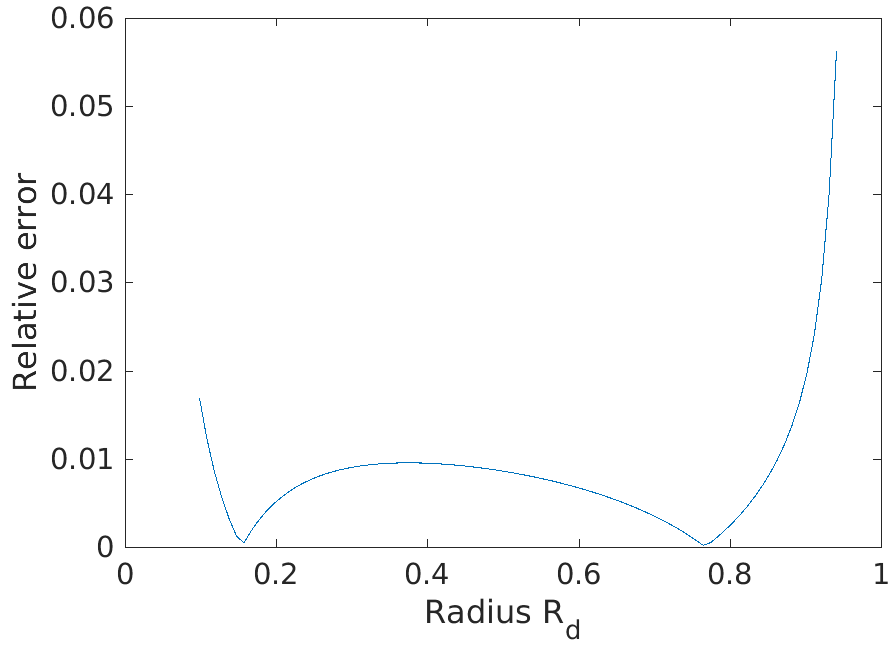
\includegraphics[scale=0.5]{../Model_problem/simpleErr.png}
	\caption{Relative error between integral formulation and multipole expansion solutions for different defect radius $R_d$.}
	\label{fig:simpleErr}
\end{minipage}
\end{figure}

Figure \ref{fig:simpleSol} shows the resonance frequency of the model problem, the resonance frequency of the small bubble in free-space and the resonance frequency of the Dirichlet problem on the big bubble without the inclusion. It can be seen that the resonance frequency of the model problem is higher compared to the bubble in free-space. For $R_d \rightarrow R_b$, the system behaves like a Dirichlet problem for the Helmholtz equation on the small bubble, and the resonance frequency tends to the first eigenvalue of this problem.

Figure \ref{fig:simpleErr} shows the relative error between the solutions using the integral operator and the multipole expansions methods. For intermediate $R_d$, the relative error is of the order $1\%$, so the two methods agree.

The conclusion is that we also have resonance in the model problem, and that the resonance frequency is higher compared to the free-space bubble. This suggests that there will be a resonance mode corresponding to the small bubble in the full problem, and that this resonance frequency will lie in the bandgap of the crystal.

\section{Numerical implementation}
We seek a spatial discretization of the boundary integral formulation. The factors $\Scrystal$ and $\KstarC$ require the Green's function $G$ for the crystal, so the equation \eqnref{eq:G} has to be solved numerically. We will apply the method found in \cite{bandgap}.

Applying the Floquet transform we can decompose $G$ into the $\alpha$-quasiperiodic Green's function $G_\alpha$ which satisfies
\begin{equation*}
\Delta G_\alpha + (k^2+(k_b^2-k^2)\chi(\C))G_\alpha = \sum_{n\in \Z} \delta(x-y-n)e^{in\cdot\alpha}.
\end{equation*}
Here $\alpha$ is in the so called first Brillouin zone $[0,2\pi]^2$. Let $Y= [-1/2,1/2]^2$. For a fixed $y\in \R^2$, the function $u(x)=G_\alpha(x,y)$ is a solution to the problem
\begin{equation} \label{eq:quasiperiodic}
\left\{
\begin{array} {ll}
&\ds \nabla \cdot \frac{1}{\rho} \nabla  u+ \frac{\omega^2}{\kappa} u  = \delta(x-y) \quad \text{in} \quad Y \backslash  \bar{D}, \\
\nm
&\ds \nabla \cdot \frac{1}{\rho_b} \nabla  u+ \frac{\omega^2}{\kappa_b} u  = \delta(x-y) \quad \text{in} \quad D, \\
\nm
&\ds  u_{+} -u_{-}  =0   \quad \text{on} \quad \partial D, \\
\nm
& \ds  \frac{1}{\rho} \frac{\partial u}{\partial \nu} \bigg|_{+} - \frac{1}{\rho_b} \frac{\partial u}{\partial \nu} \bigg|_{-} =0 \quad \text{on} \quad \partial D, \\
&  e^{-i \alpha \cdot x} u  \,\,\,  \text{is periodic.}
\end{array}
\right.
\end{equation}
Because of the reciprocity relation $G_\alpha(x,y) = G_\alpha(y,x)$, also $e^{-i \alpha \cdot y} G_\alpha(x,y)$ is periodic in $y$, so we can restrict to the case $y\in Y$. Let $\Gamma_\alpha^k$ be the quasi-periodic Green's function, defined as the solution to the equation
\begin{equation*}
\Delta \Gamma_\alpha^k(x,y) + k^2\Gamma_\alpha^k(x,y) = \sum_{n\in \Z} \delta(x-y-n)e^{in\cdot\alpha}.
\end{equation*}
This Green's function can be expanded as
\begin{equation} \label{eq:quasihomogenious}
\Gamma_\alpha^k(x,y) = -\frac{i}{4}\sum_{m\in \Z^2} H_0(k|x-y-m|)e^{im\cdot\alpha}.
\end{equation}
The function $G_\alpha-\Gamma_\alpha^k$ satisfies \eqnref{eq:quasiperiodic} without the Dirac mass, so we can write
\begin{equation} \label{eq:G_a}
G_\alpha(x,y) = \begin{cases} \Gamma_\alpha^{k_b}(x,y) + S_D^{k_b}[\psi_b](x) \quad &x\in D, \\  \Gamma_\alpha^{k}(x,y) + S_D^{\alpha,k}[\psi](x) &x\in Y \backslash \bar{D} \end{cases}.
\end{equation}
Using the jump relations for the single layer potentials, we find that
\begin{equation*}
\B(\omega,\delta)[\Psi] = F,
\end{equation*}
where 
\begin{equation*}
\B(\omega, \delta) = 
\begin{pmatrix}
\S_D^{k_b} &  -\S_D^{\alpha,k}  \\
-\frac{1}{2}+ \K_D^{k_b, *}& -\delta( \frac{1}{2}+ (\K_D^{ -\alpha,k})^*)
\end{pmatrix}, 
\,\, \Psi= 
\begin{pmatrix}
\psi_b\\
\psi
\end{pmatrix},
\,\, F=
\begin{pmatrix}
\Gamma_\alpha^{k} - \Gamma_\alpha^{k_b} \\
\delta\frac{\partial \Gamma_\alpha^{k}}{\partial \nu} -
\frac{\partial \Gamma_\alpha^{k_b}}{\partial \nu} 
\end{pmatrix}.
\end{equation*}
The method in \cite{bandgap} discretizes this system using the Fourier basis $e^{in\theta}$, so  we need to expand the function $\Gamma_\alpha^k(x,y)$ in terms of the polar coordinates $(r,\theta)$ of $x$. We will use the following version of Graf's addition theorem.

\begin{equation*}
H_l^{(1)}(kr_2)e^{il\theta_2} =
\begin{cases}
\sum_{n=-\infty}^\infty H_{l-n}(kb)e^{i(l-n)\beta}J_n(kr_1)e^{in\theta_1} \qquad &\text{if } r_1<b, \\
\sum_{n=-\infty}^\infty H_{l-n}(kr_1)e^{i(l-n)\theta_1}J_n(kb)e^{in\beta} \qquad &\text{if } r_1>b.
\end{cases}
\end{equation*}
In these equations, we have $x_1 = r_1e^{i\theta_1}, x_2 = r_2e^{i\theta_2}$ and $x_2 = x_1 + be^{i\beta}$. 

In the following, pick $x$ on the boundary $\partial D$, i.e. $x = R_be^{i\theta}$. Furthermore, pick $y=r'e^{i\theta'}$ inside $Y$. Using the addition formulas, we have
\begin{align*}
H_0^{(1)}(k|x-y-m|) &= 
\begin{cases}
\sum_{n=-\infty}^\infty (-1)^nH_{-n}(k|y+m|)e^{-in\theta_m'}J_n(kR_b)e^{in\theta} \qquad &\text{if } R_b<|y+m|, \\
\sum_{n=-\infty}^\infty (-1)^nH_{-n}(kR_b)e^{-in\theta}J_n(k|y+m|)e^{in\theta_m'} \qquad &\text{if } R_b>|y+m|.
\end{cases}
\end{align*}
For $m\neq 0$ we have $R_b<|y+m|$ and
\begin{equation*}
H_{-n}(k|y+m|)e^{-in\theta_m'} = \sum_{l=-\infty}^\infty H_{-n-l}(k|m|)e^{i(-n-l)\theta_m}J_l(kr')e^{il\theta'}.
\end{equation*}
Plugging in above expressions into \eqnref{eq:quasihomogenious}, we find
\begin{equation*}
\Gamma_\alpha^k(x,y) = -\frac{i}{4}\sum_{n=-\infty}^\infty\left[ M_ne^{in\theta} + \sum_{l=-\infty}^\infty\left[ \sum_{m\in \Z^2, m\neq 0} H_{-n-l}(k|m|)e^{i(-n-l)\theta_m}e^{im\cdot\alpha} \right] (-1)^nJ_l(kr')e^{il\theta'}J_n(kR_b)e^{in\theta}\right],
\end{equation*}
where the terms $M_n$, corresponding to $m=0$, are given by
\begin{equation*}
M_n = \begin{cases}
(-1)^nH_{-n}(kr')e^{-in\theta'}J_n(kR_b) \quad &\text{if } r' > R_b \\
(-1)^nH_{n}(kR_b)J_{-n}(kr')e^{-in\theta'} \quad &\text{if } r' < R_b.
\end{cases}
\end{equation*}
The two different cases correspond to the source $y$ being inside or outside the bubble. Define the lattice sum $Q_n$ as 
\begin{equation*}
Q_n = \sum_{m\in \Z^2, m\neq 0} H_{n}(k|m|)e^{in\theta_m}e^{im\cdot\alpha}.
\end{equation*}
Then the expression for $\Gamma_\alpha^k$ is 
\begin{equation}\label{eq:gammafourier}
\Gamma_\alpha^k(x,y) = -\frac{i}{4}\sum_{n=-\infty}^\infty\left[ M_n + \sum_{l=-\infty}^\infty Q_{-n-l} (-1)^nJ_l(kr')e^{il\theta'}J_n(kR_b)\right]e^{in\theta}.
\end{equation}
This can be viewed as a Fourier series expansion of $\Gamma_\alpha^k$ as a function of $x\in S^1$. The $n$:th Fourier coefficient is
\begin{equation*}
-\frac{i}{4}\left[M_n + \sum_{l=-\infty}^\infty Q_{-n-l} (-1)^nJ_l(kr')e^{il\theta'}J_n(kR_b)\right].
\end{equation*}
We also need the Fourier coefficients of $\frac{\partial \Gamma_\alpha^k}{\partial \nu(x)}$.  For $x\in \partial D$ we have
\begin{equation*}
\frac{\partial \Gamma_\alpha^k}{\partial \nu(x)} = \frac{\partial \Gamma_\alpha^k}{\partial r} \Bigg|_{r=R_b}.
\end{equation*} 
Differentiating equation \ref{eq:gammafourier} we find
\begin{equation*}
\frac{\partial \Gamma_\alpha^k}{\partial \nu(x)} = -\frac{i}{4}\sum_{n=-\infty}^\infty\left[ M_n' + \sum_{l=-\infty}^\infty Q_{-n-l} (-1)^nJ_l(kr')e^{il\theta'}kJ_n'(kR_b)\right]e^{in\theta},
\end{equation*}
where
\begin{equation*}
M_n' = \begin{cases}
(-1)^nkH_{-n}(kr')e^{-in\theta'}J_n'(kR_b) \quad &\text{if } r' > R_b, \\
(-1)^nkH'_{n}(kR_b)J_{-n}(kr')e^{-in\theta'} \quad &\text{if } r' < R_b.
\end{cases}
\end{equation*}
The system \eqnref{eq:G_a} is discretized by truncating these sums, and is solved to find $G_\alpha(x,y)$. The Green's function $G$ is then found using the formula
\begin{equation*}
G(x,y) = \frac{1}{(2\pi)^2}\int_{[0,2\pi]^2} G_\alpha(x,y) \dx \alpha,
\end{equation*}
i.e. $G$ is the average of $G_\alpha$ over the first Brillouin zone. The operators $\Scrystal$ and $\KstarC$ are then discretized using Nyström's method, and the characteristic values of $\A$ inside the bandgap are computed using Muller's method. \cite{first}

\section{Asymptotic expansions as $\epsilon \rightarrow 0$}
In this section we give asymptotic expansions of the operators as the perturbation $\epsilon$ of the radius tends to zero. Let $x,y\in \partial D$ and let $\tilde{x} = x - \epsilon \nu(x) \in \partial D_d$. For a layer density $\phi$ on $\partial D$, define $\tilde{\phi}$ on $\partial D_d$ by $\tilde{\phi}(\tilde{x}) = \phi (x)$. We begin with the expansions of the operators $\S_{D_d}, \S_{D,D_d}$ and  $\S_{D_d,D}$. 

\begin{prop}\label{prop:asympsingle}
	Let $\phi \in L^2(\partial D)$ and let $x,y,\tilde{x},\tilde{y},\tilde{\phi}$ be as above. Then 
\begin{equation} \label{eq:asympSdD}
\S_{D_d,D}^k[\phi](\tilde{x}) = \S_D^k[\phi](x) -\epsilon \left(-\frac{1}{2}I + \left(\K_D^k\right)^*\right)[\phi](x) + o(\epsilon),
\end{equation}
\begin{equation} \label{eq:asympSd}
\S_{D_d}^k[\tilde{\phi}](\tilde{x}) = \S_D^k[\phi](x) - \epsilon \left(\frac{1}{R_b}\S_D^k + \K_D^k + \left(\K_D^k\right)^*\right)[\phi](x) + o(\epsilon)
\end{equation}
\begin{equation} \label{eq:asympSDd}
\S_{D,D_d}^k[\tilde{\phi}](x) = \S_D^k[\phi](x) - \epsilon \left(-\frac{1}{2}I+ \frac{1}{R_b}\S_D^k + \K_D^k \right)[\phi](x) + o(\epsilon)
\end{equation}
where the $o(\epsilon)$-terms depend on $\|\phi\|_{L^2(\partial D)}$.
\end{prop}
Here the $o(\epsilon)$ terms are in the $L^2$ sense, i.e. for any fixed $\phi$ we have 
\begin{equation*}
	\lim_{\epsilon \rightarrow 0} \frac{1}{\epsilon}\left\| \S_{D_d,D}^k[\phi](\tilde{x}) -\left( \S_D^k[\phi](x) -\epsilon \left(-\frac{1}{2}I + \left(\K_D^k\right)^*\right)[\phi]\right) \right\|_{L^2(\partial D)} = 0,
\end{equation*}
and similarly for the other expansions.
\begin{proof}
The proof is given in \cite{asymptotics}, but in our case with the Taylor expansions in the $L^2$ sense (as given in \cite{weakdifffcn}, Theorem 3.4.2).
\end{proof}
\begin{prop} \label{prop:asympK}
	Let $\phi \in L^2(\partial D)$ and let $x,y,\tilde{x},\tilde{y},\tilde{\phi}$ be as above. Then 
	\begin{equation} \label{eq:asympK}
	\left(\K_{D_d}^k\right)^*[\tilde{\phi}](\tilde{x}) = \left(\K_{D}^k\right)^*[\phi](x) - \epsilon \left(\frac{1}{R_b}\left(\K_D^k\right)^* +\K_1\right) + \O(\epsilon^2),
	\end{equation}
	where $\K_1$ is given by
	\begin{equation}
	\K_1^k = \frac{k^2}{R_b} \int_{\partial D} \langle x-y,\nu_x \rangle H_0''(k|x-y|)\phi(y)\dx \sigma(y),
	\end{equation}
	and the $\O(\epsilon^2)$-term depends on $\|\phi\|_{L^2}$.
\end{prop}
\begin{proof}
The explicit expansion of $\K_{D_d}^*$ is derived in \cite{lecturenotes} for the Laplace case. We compute this in our case using similar arguments. Because $\partial D$ and $\partial D_d$ are circles, we have
\begin{equation} \label{eq:dsigma}
\dx \sigma(\tilde{y}) = \left( 1-\frac{\epsilon}{R_b} \right) \dx \sigma(y).
\end{equation}
Furthermore, again using that the boundaries are circles, we have
\begin{align*}
\frac{\partial}{\partial \nu_{\tilde{x}}} H_0(k|\tilde{x}-\tilde{y}|) &= kH_0'(k|\tilde{x}-\tilde{y}|)\frac{\langle \tilde{x}-\tilde{y},\nu_{\tilde{x}} \rangle}{|\tilde{x}-\tilde{y}|} \\
&= kH_0'(k|\tilde{x}-\tilde{y}|)\frac{\langle x-y,\nu_{x} \rangle}{|x-y|}
\end{align*}
and
\begin{align*}
H_0'(k|\tilde{x}-\tilde{y}|) &= H_0'\left(k|x-y|\left( 1-\frac{\epsilon}{R_b} \right)\right) \\
&= H_0'\left(k|x-y|\right) - \frac{\epsilon}{R_b}k|x-y|H_0''\left(k|x-y|\right) + \O(\epsilon^2).
\end{align*} 
It follows that 
\begin{align*}
\left(\K_{D_d}^k\right)^*[\tilde{\phi}](\tilde{x}) &= \int_{D_d} \frac{\partial}{\partial \nu_{\tilde{x}}} H_0'(k|\tilde{x}-\tilde{y}|) \tilde{\phi}({\tilde{y}}) \dx\sigma(\tilde{y}) \\
&= \int_{D} k\left( H_0'\left(k|x-y|\right) - \frac{\epsilon}{R_b}k|x-y|H_0''\left(k|x-y|\right) \right)\frac{\langle x-y,\nu_{x} \rangle}{|x-y|} \left( 1-\frac{\epsilon}{R_b} \right) \phi(y)\dx\sigma(y) + \O(\epsilon^2) \\
&= \int_{D} k H_0'\left(k|x-y|\right)\frac{\langle x-y,\nu_{x} \rangle}{|x-y|} \dx \sigma(y) \\
& \quad -\epsilon \left[\frac{1}{R_b}\int_{D} k H_0'\left(k|x-y|\right)\frac{\langle x-y,\nu_{x} \rangle}{|x-y|} \dx \sigma(y) + \frac{k^2}{R_b} \int_{\partial D} \langle x-y,\nu_x \rangle H_0''(k|x-y|)\phi(y)\dx \sigma(y) \right] \\
& \quad + \O(\epsilon^2),
\end{align*}
and hence
\begin{equation*}
\left(\K_{D_d}^k\right)^*[\tilde{\phi}](\tilde{x}) = \left(\K_{D}^k\right)^*[\phi](x) - \epsilon \left(\frac{1}{R_b}\left(\K_D^k\right)^* +\K_1\right)[\phi](x) + \O(\epsilon^2).
\end{equation*}
\end{proof}
\begin{prop} \label{prop:asympderiv}
	Let $\phi \in H^1(\partial D)$ and let $x,y,\tilde{x},\tilde{y},\tilde{\phi}$ be as above. Then 
\begin{equation} \label{eq:asymppSdD}
\frac{\partial \S_{D_d,D}^k[\phi]}{\partial \tilde{\nu}} (\tilde{x}) = \left(-\frac{1}{2}I + \left(\K_D^k\right)^*\right)[\phi](x) - \epsilon \mathcal{R}_D^k[\phi](x) + o(\epsilon),
\end{equation}
\begin{equation} \label{eq:asymppSDd}
\frac{\partial \S_{D,D_d}^k[\tilde{\phi}]}{\partial \nu} (x) = \left(\frac{1}{2}I + \left(\K_D^k\right)^*\right)[\phi](x) - \epsilon \L_D^k[\phi](x) + o(\epsilon),
\end{equation}
where $\mathcal{R}_D^k$ and $\L_D^k$ are given by
\begin{equation*}
\mathcal{R}_D^k = -k^2\S_D^k + \frac{1}{R_b} \left(-\frac{1}{2}I + \left(\K_D^k\right)^*\right) -\frac{\partial^2}{\partial T^2}\S_D^k,
\end{equation*}
\begin{equation*}
\L_D^k = \frac{1}{R_b} \left(\frac{1}{2}I + \left(\K_D^k\right)^*\right) +\frac{\partial \D_D^k}{\partial \nu},
\end{equation*}
and the $o(\epsilon)$-terms depend on $\|\phi\|_{L^2(\partial D)}$. Here $\frac{\partial^2}{\partial T^2}$ denotes the tangential derivative. 
\end{prop}
\begin{proof}
The proof is similar to the one given in \cite{asymptoticsderivative}. Because $\phi\in H^1(\partial D)$ we have that $\S_D^k[\phi]\in H^2(\partial D)$. Because the normals $\tilde{\nu}_{\tilde{x}}$ and $\nu_x$ coincide, we have
\begin{align*}
\frac{\partial \S_{D_d,D}^k[\phi]}{\partial \tilde{\nu}} (\tilde{x}) &= \nu \cdot \nabla \S_{D_d,D}^k[\phi](\tilde{x}) \\
&= \frac{\partial \S_D^k[\phi]}{\partial \nu} \bigg|_{-}(x) - \epsilon\left(\frac{\partial^2}{\partial \nu^2}\S_D^k[\phi]\bigg|_{-}(x) \right) + o(\epsilon)
\end{align*}
Using the Laplacian in polar coordinates
\begin{equation*}
\Delta = \frac{\partial^2}{\partial r^2} + \frac{1}{r}\frac{\partial}{\partial r} + \frac{1}{r^2}\frac{\partial^2}{\partial \theta^2},
\end{equation*}
together with the relation $\frac{1}{r^2}\frac{\partial^2}{\partial \theta^2} = \frac{\partial^2}{\partial T^2}$, we find
\begin{equation*}
\frac{\partial^2}{\partial \nu^2}\S_D^k[\phi]\bigg|_{-}(x) = -k^2\S_D^k[\phi](x) -\frac{1}{R_b}\frac{\partial \S_D^k[\phi]}{\partial \nu}\bigg|_{-}(x) - \frac{\partial^2 \S_D^k[\phi]}{\partial T^2}(x),
\end{equation*}
so equation \eqnref{eq:asymppSdD} follows using the jump relations. To derive equation \eqnref{eq:asymppSDd}, pick a function $f\in H^1(\partial D)$. Then there exists a solution $u$ to the exterior Dirichlet problem
\begin{equation*}
\begin{cases}
\Delta u + k^2 u = 0 \quad &\text{in } \R^2\setminus D \\
u = f & \text{in } \partial D \\
u \text{ satisfies the So} &\hspace{-10pt}\text{mmerfeld radiation condition}
\end{cases}
\end{equation*}
Using duality and integration by parts in the exterior region, we obtain that
\begin{align*}
\int_{\partial D} \frac{\partial \S_{D,D_d}^k[\tilde{\phi}]}{\partial \nu} (x) f(x) \dx \sigma(x) &= \int_{\partial D} \S_{D,D_d}^k[\tilde{\phi}](x)\frac{\partial f }{\partial \nu} (x)  \dx \sigma(x) \\
&= \int_{\partial D_d} \S_{D_d,D}^k\left[\frac{\partial f }{\partial \nu}\right](\tilde{x})\tilde{\phi}(\tilde{x}) \dx \sigma(\tilde{x}).
\end{align*}
Combining Proposition \ref{prop:asympsingle} together with \eqnref{eq:dsigma} we find
\begin{align*}
\int_{\partial D_d} \S_{D_d,D}^k\left[\frac{\partial f }{\partial \nu}\right](\tilde{x})\tilde{\phi}(\tilde{x}) \dx \sigma(\tilde{x}) &= \int_{\partial D}\left( \S_D^k\left[\frac{\partial f }{\partial \nu}\right] (x) -\epsilon \left(-\frac{1}{2}I + \left(\K_D^k\right)^*\right)\left[\frac{\partial f }{\partial \nu}\right](x)\right)\phi(x)\left(1-\frac{\epsilon}{R_b}\right)\dx \sigma(x) + o(\epsilon) \\
&= \int_{\partial D}\S_D^k\left[\frac{\partial f }{\partial \nu}\right] \phi\dx \sigma -\epsilon \int_{\partial D}\left( \frac{1}{R_b}\S_D^k -\frac{1}{2}I + \left(\K_D^k\right)^*\right)\left[\frac{\partial f }{\partial \nu}\right]\phi\dx \sigma + o(\epsilon) \\
& = \int_{\partial D} \S_D^k\left[\phi\right]\frac{\partial f }{\partial \nu} \dx \sigma -\epsilon \int_{\partial D}\left( \frac{1}{R_b}\S_D^k -\frac{1}{2}I + \K_D^k\right)\left[\phi\right]\frac{\partial f }{\partial \nu}\dx \sigma + o(\epsilon) \\
&= \int_{\partial D} \frac{\partial \S_D^k }{\partial \nu}[\phi]\bigg|_{+}f \dx \sigma -\epsilon \int_{\partial D}\left(\frac{1}{R_b}\frac{\partial \S_D^k }{\partial \nu}\bigg|_{+} +\frac{\partial \D_D^k}{\partial \nu} \right)\left[\phi\right]f\dx \sigma + o(\epsilon).
\end{align*}
Therefore \eqnref{eq:asymppSDd} follows using the jump formulas.
\end{proof}


Using the asymptotic expansions \eqnref{eq:asympSdD}, \eqnref{eq:asympSd}, \eqnref{eq:asympSDd}, \eqnref{eq:asympK}, \eqnref{eq:asymppSdD} and \eqnref{eq:asymppSDd}, we can expand the operator $\A$ as 
\begin{equation}
\A = \A_0 - \epsilon \A_1 + o(\epsilon),
\end{equation}
where
\begin{equation} \label{eq:A0}
\A_0 = 
\begin{pmatrix}
\S_{D}^{k_b} &  -\S_{D}^{k} & -\S_{D}^{k} & 0 \\
0 & \S_{D}^k & \S_{D}^k & -\Scrystal \\
-\frac{1}{2}I+ (\K_{D}^{k_b})^*& -\delta\left( \frac{1}{2}I+ (\K_{D}^{k})^*\right) & -\delta\left( -\frac{1}{2}I+ (\K_{D}^{k})^*\right) & 0 \\
0 & \frac{1}{2}I+ (\K_D^{k})^* & -\frac{1}{2}I+ (\K_D^{k})^* & -\left( \frac{c}{2}I+ \left(\K_D^{\#,+}\right)^*\right)
\end{pmatrix}, 
\end{equation}
and
\begin{equation} \label{eq:A1}
\A_1 = 
\begin{pmatrix}
\frac{1}{R_b}\S_D^{k_b} + \K_D^{k_b} + \left(\K_D^{k_b}\right)^* &  -\frac{1}{R_b}\S_D^{k_b} - \K_D^{k} - \left(\K_D^{k}\right)^* & \frac{1}{2}I - \left(\K_D^k\right)^* & 0 \\
0 & -\frac{1}{2}I+ \frac{1}{R_b}\S_D^k + \K_D^k  & 0 & 0 \\
\K_1^{k_b}& -\delta\left(\frac{1}{R_b}\left(\K_D^k\right)^* + \K_1^k\right) & -\delta \mathcal{R}_D^k  & 0 \\
0 & \L_D^k & 0 & 0
\end{pmatrix}.
\end{equation}
Using elementary row reductions, these operators are equivalent to 
\begin{equation}
\hat{\A} = \hat{\A}_0 - \epsilon \hat{\A}_1 + o(\epsilon),
\end{equation}
where
\begin{equation} \label{eq:Ahat0}
\hat{\A}_0 = 
\begin{pmatrix}
\S_{D}^{k_b} &  0 & 0 & -\Scrystal \\
0 & \S_{D}^k & \S_{D}^k & -\Scrystal \\
-\frac{1}{2}I+ (\K_{D}^{k_b})^* & 0 & 0 & -\delta\left( \frac{c}{2}I+ \left(\K_D^{\#,+}\right)^*\right)\\
0 & \frac{1}{2}I+ (\K_D^{k})^* & -\frac{1}{2}I+ (\K_D^{k})^* & -\left( \frac{c}{2}I+ \left(\K_D^{\#,+}\right)^*\right)
\end{pmatrix}, 
\end{equation}
and
\begin{equation} \label{eq:Ahat1}
\hat{\A}_1 = 
\begin{pmatrix}
\frac{1}{R_b}\S_D^{k_b} + \K_D^{k_b} + \left(\K_D^{k_b}\right)^* &  -\frac{1}{2}I - \left(\K_D^k\right)^* & \frac{1}{2}I - \left(\K_D^k\right)^* & 0 \\
0 & -\frac{1}{2}I+ \frac{1}{R_b}\S_D^k + \K_D^k  & 0 & 0 \\
\K_1^{k_b} & -\delta\left(-\frac{1}{2R_b}I-\frac{\partial\D_D^k}{\partial \nu}+\K_1^k\right) & -\delta \mathcal{R}_D^k & 0 \\
0 & \L_D^k & 0 & 0
\end{pmatrix}.
\end{equation}
The first and third row of $\hat{\A}_0$ decouples, and we obtain the matrix
\begin{equation*}
\begin{pmatrix}
\S_{D}^{k_b} & -\Scrystal \\
-\frac{1}{2}I+ (\K_{D}^{k_b})^* & -\delta\left( \frac{c}{2}I+ \left(\K_D^{\#,+}\right)^*\right)\\
\end{pmatrix}, 
\end{equation*}
which clearly corresponds to the unperturbed crystal. 

\section{simplifications}

We have
\begin{equation*}
\frac{|x-y|}{R_b}=2\frac{\langle x-y,\nu_x\rangle}{|x-y|},
\end{equation*}
so we can rewrite the expression for $\K_1^k$ as 
\begin{equation*}
\K_1^k[\phi](x) = \int_{\partial D} 2k^2 \frac{\langle x-y,\nu_x\rangle^2}{|x-y|^2} H_0''(k|x-y|) \phi(y) \dx (y).
\end{equation*}
Furthermore, since $|x-y|=\langle x-y, \nu_x \rangle^2 + \langle x-y, T_x \rangle^2 $, we obtain
\begin{equation*}
\K_1^k[\phi](x) = \int_{\partial D} 2k^2 \left(1- \frac{\langle x-y,T_x\rangle^2}{|x-y|^2} \right)H_0''(k|x-y|) \phi(y) \dx\sigma (y).
\end{equation*}

Using the relation
\begin{equation*}
H_0''(x) = -H_0(x)-\frac{1}{x}H_0'(x)
\end{equation*}
we can rewrite the expression for $\frac{\partial^2 \S_D^k[\phi]}{\partial T^2}(x)$. We have
\begin{equation*}
\frac{\partial^2}{\partial T^2}H_0(k|x-y|) = k^2\frac{\langle x-y, T_x\rangle^2}{|x-y|^2}H_0''(k|x-y|) + k \left(\frac{1}{|x-y|} -\frac{1}{R}\frac{\langle x-y,\nu_x\rangle }{|x-y|} -\frac{\langle x-y, T_x\rangle^2}{|x-y|^3} \right) H_0'(k|x-y|),
\end{equation*}
and hence 
\begin{equation*}
\frac{\partial^2}{\partial T^2}H_0(k|x-y|) = \left(2k^2\frac{\langle x-y, T_x\rangle^2}{|x-y|^2 }-k^2\right)H_0''(k|x-y|) -\frac{k}{R}\frac{\langle x-y,\nu_x\rangle }{|x-y|}H_0'(k|x-y|) - k^2 \left(1 -\frac{\langle x-y, T_x\rangle^2}{|x-y|^2} \right)H_0(k|x-y|),
\end{equation*}

\bibliography{defect}{}
\bibliographystyle{plain}
\end{document}
